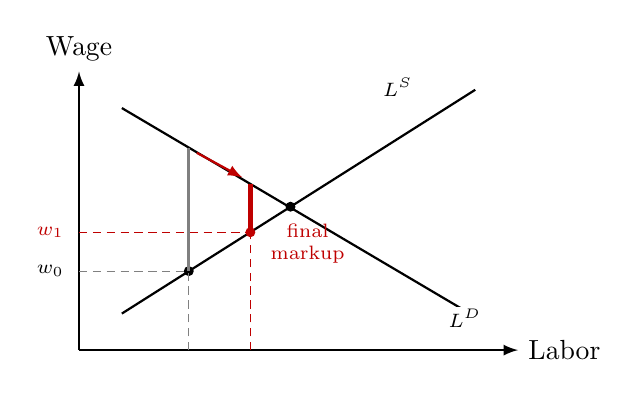
\begin{tikzpicture}[x=0.68cm,y=0.58cm,>=latex]
    \draw[->,thick] (0,0) -- (8.2,0) node[right] {Labor};
    \draw[->,thick] (0,0) -- (0,6.1) node[above] {Wage};

    % Labor supply and labor demand
    \draw[thick] (0.8,0.8) -- (7.4,5.7)
        node[pos=0.88,above left=6pt,font=\scriptsize,fill=white,inner sep=1pt] {$L^S$};
    \draw[thick] (0.8,5.3) -- (7.3,0.8)
        node[pos=0.88,below right=6pt,font=\scriptsize,fill=white,inner sep=1pt] {$L^D$};

    % Competitive equilibrium
    \coordinate (Ecompetitive) at (3.95,3.14);
    \fill (Ecompetitive) circle (1.8pt);

    % Initial high-markup quantity and wage (the wage lies on labor supply).
    \coordinate (LinitialDemand) at (2.05,4.43);
    \coordinate (LinitialSupply) at (2.05,1.73);
    \fill (LinitialSupply) circle (1.8pt);
    \draw[densely dashed,gray] (0,1.73) -- (LinitialSupply)
        node[pos=0,left=2pt,font=\scriptsize,text=black] {$w_0$};
    \draw[densely dashed,gray] (2.05,0) -- (LinitialDemand);

    % Lower markup: employment moves right and the wage rises along labor supply.
    \coordinate (LfinalDemand) at (3.20,3.64);
    \coordinate (LfinalSupply) at (3.20,2.58);
    \fill[red!75!black] (LfinalSupply) circle (1.8pt);
    \draw[densely dashed,red!75!black] (0,2.58) -- (LfinalSupply)
        node[pos=0,left=2pt,font=\scriptsize,text=red!75!black] {$w_1$};
    \draw[densely dashed,red!75!black] (3.20,0) -- (LfinalDemand);
    \draw[->,red!75!black,thick] (2.20,4.32) -- (3.05,3.78);

    % The markup is the wedge between labor demand and labor supply.
    \draw[gray,line width=1.2pt] (LinitialSupply) -- (LinitialDemand);
    \draw[red!75!black,line width=2pt] (LfinalSupply) -- (LfinalDemand)
        node[midway,right=3pt,yshift=-13pt,font=\scriptsize,align=center,text=red!75!black]
        {final\\markup};
\end{tikzpicture}
